\chapter{Creating Figures}\label{Fig_Chap}
The first word in the caption of the figure should be capitalized and the rest is not. The caption of the figure should end with a period.  


\section {Regular Figure} \label{Fig_Chap_1}

The figure should be centered and the caption is left aligned. In order to cite a figure, use the following syntax: \\
\color{blue} According to Figure \ref{f1}.... \\
`F' in Figure should be capitalized even in the middle of the sentence. \color{black}


\begin{figure}[ht]
	\centering
	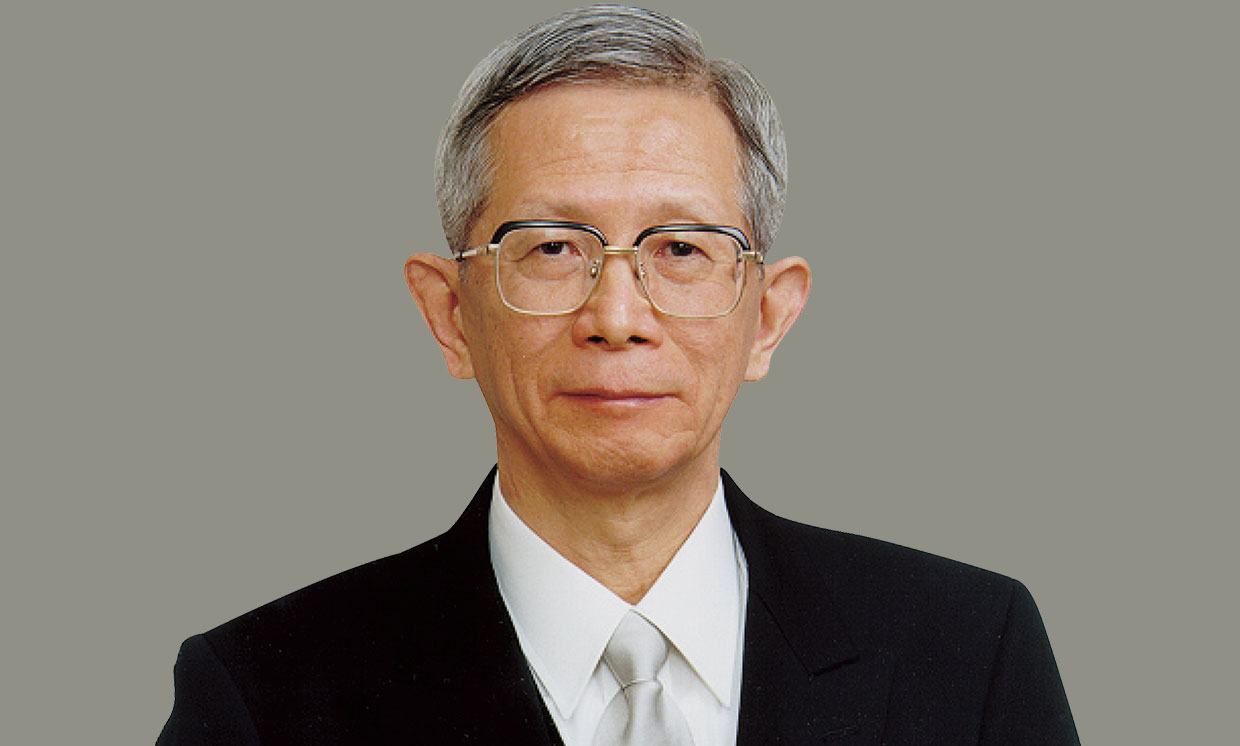
\includegraphics[width=0.5 \textwidth]{Aoyagi.jpg}	
	\caption{Dr. Takuo Aoyagi, inventor of the pulse oximeter.}
	\label{f1}       % Give a unique label
\end{figure}




\section {Figure With Caption} \label{Fig_Chap_2}

If the figure contains a source in the caption, then the source should only appear in the text but not in the table of content. \color{blue} Here is how you do it:\color{black} 


\begin{figure}[ht]
	\centering
	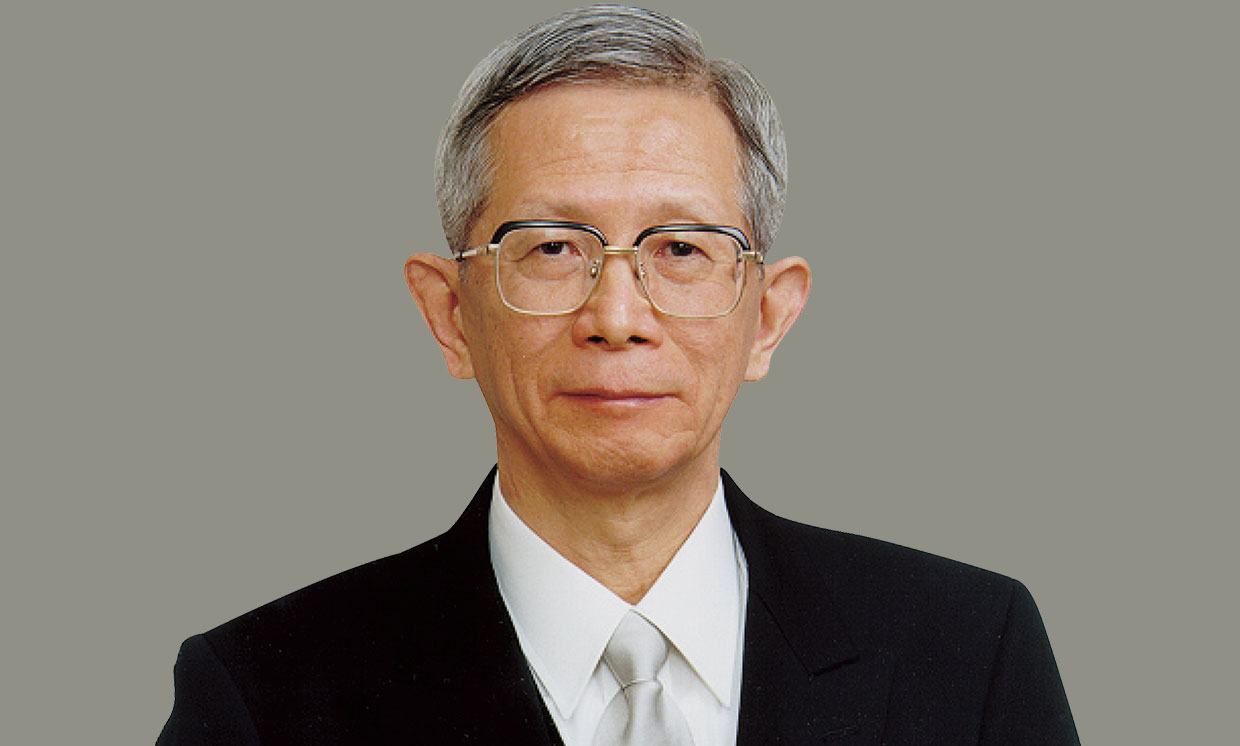
\includegraphics[width=0.5 \textwidth]{Aoyagi.jpg}	
	\caption[Dr. Takuo Aoyagi, inventor of the pulse oximeter.]{Dr. Takuo Aoyagi, inventor of the pulse oximeter. \\ \textit{\footnotesize Source: J. Goodrich, “Takuo Aoyagi, inventor of the pulse oximeter, dies at age 84,” IEEE Spectrum, 2022. [Online]. Available: https://spectrum.ieee.org/takuo-aoyagi-inventor-of- the-pulse-oximeter-dies-at-age-84. [Accessed: 20 February 2023]. }}
	\label{f2}       % Give a unique label
\end{figure}

\newpage

\section {Figure With Subplots} \label{Fig_Chap_3}

\begin{figure}[h!]
	
	\centering
	
	\begin{tabular}{c}	
		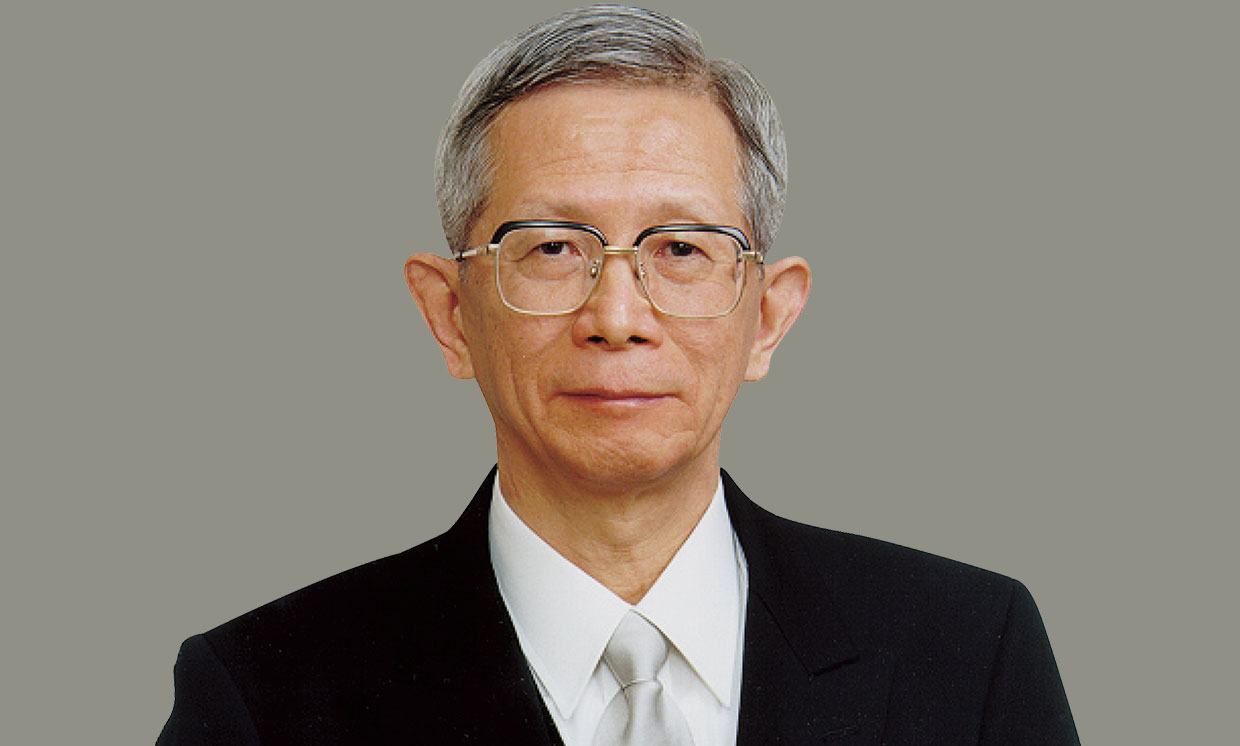
\includegraphics[width=0.5 \textwidth]{Aoyagi.jpg} \\
		(a) \\
		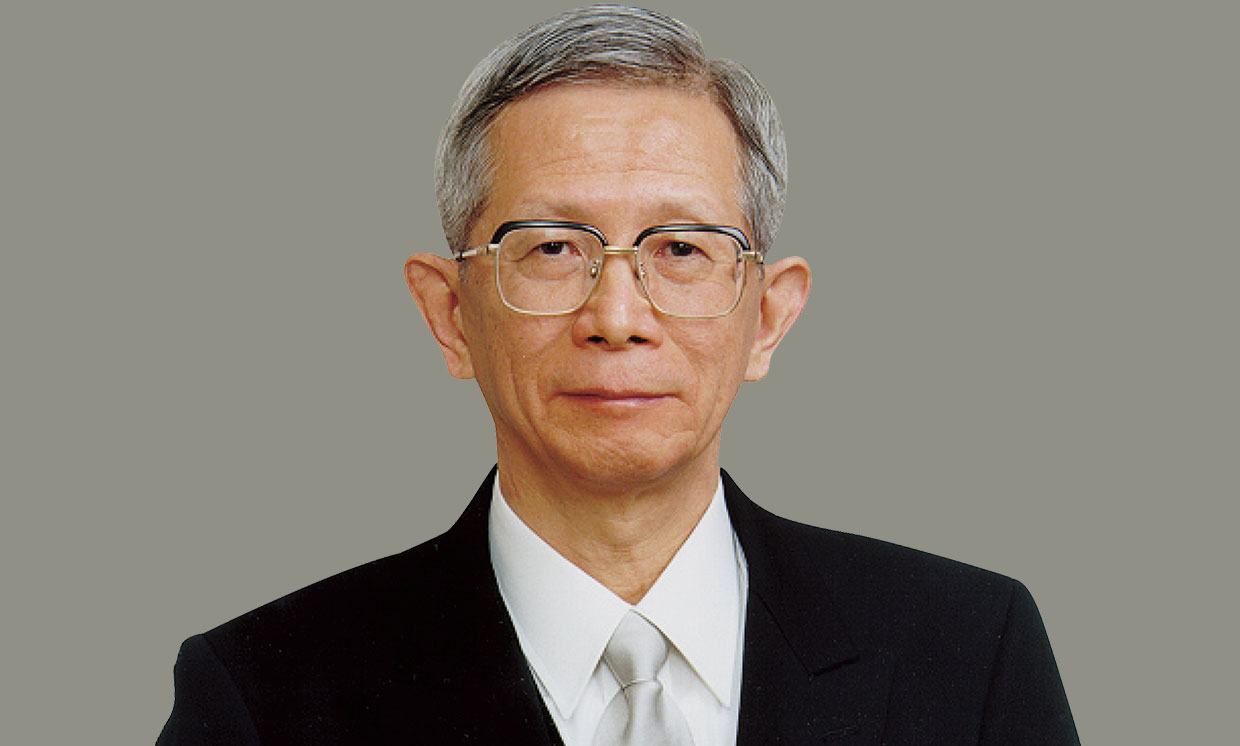
\includegraphics[width=0.5 \textwidth]{Aoyagi.jpg} \\
		(b)\\		
	\end{tabular}
	

	\caption{The subplots are atop of each other. (a) Something about subplot a. (b) Something about subplot b.}
	
	\label{f3}
\end{figure}




\begin{figure}[h!]
	
	
	\centering
	
	\begin{tabular}{cc}	
		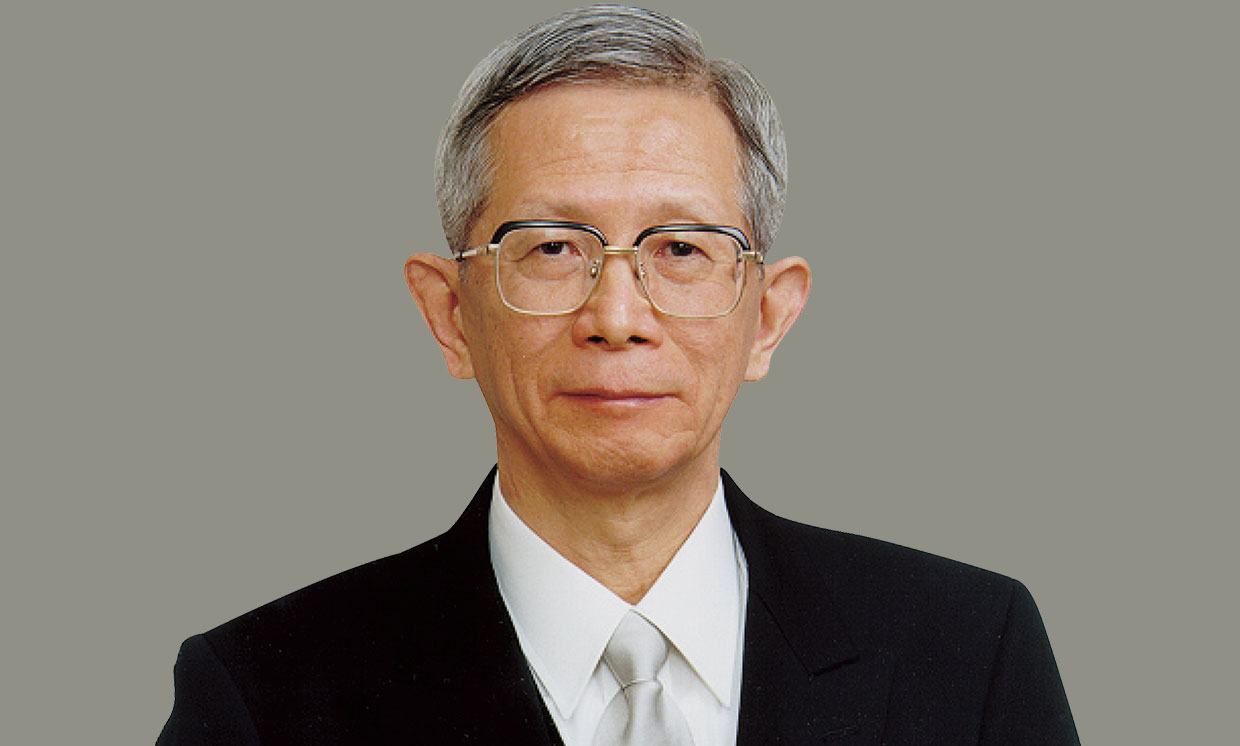
\includegraphics[width=0.35 \textwidth]{Aoyagi.jpg} & 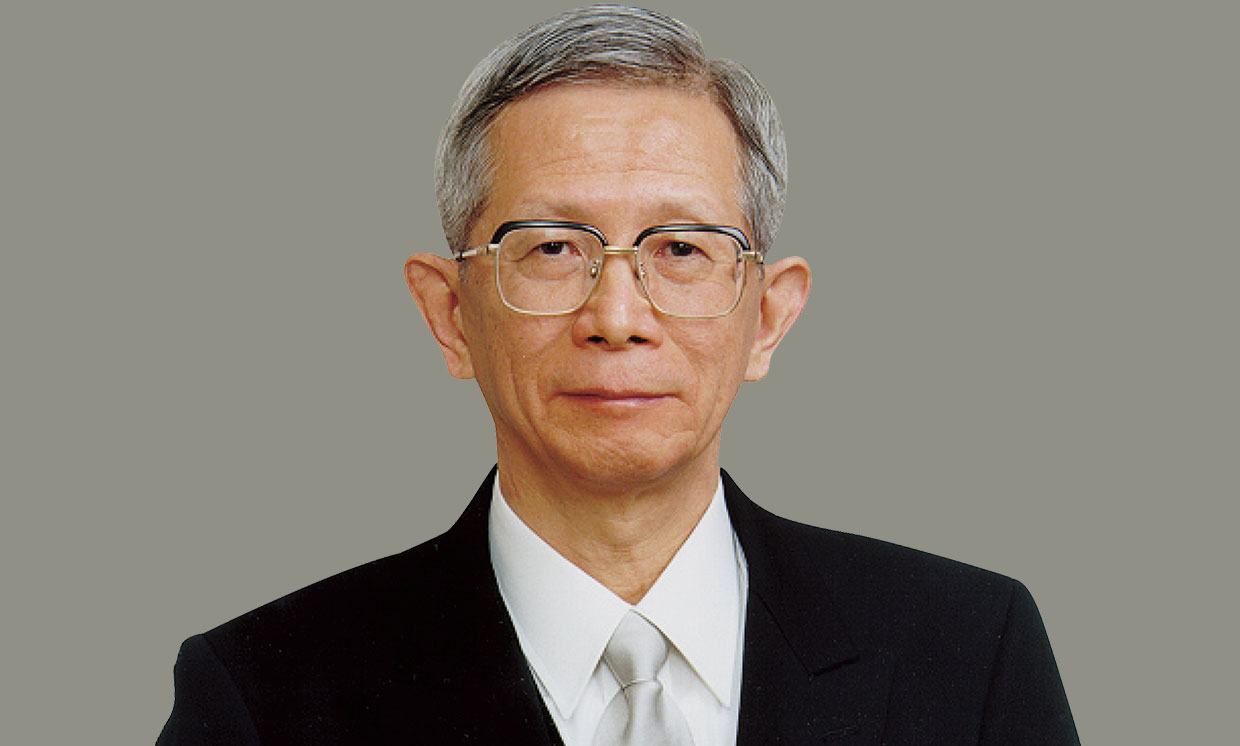
\includegraphics[width=0.35 \textwidth,angle=90]{Aoyagi.jpg}  \\
		(a)  & (b)\\		
	\end{tabular}
	
	
	\caption{The subplots are next to each other. (a) Something about subplot a. (b) Something about subplot b.}
	
	\label{f4}
\end{figure}


\section {Sideways Figure} \label{Fig_Chap_4} 

\begin{sidewaysfigure}
	\centerline{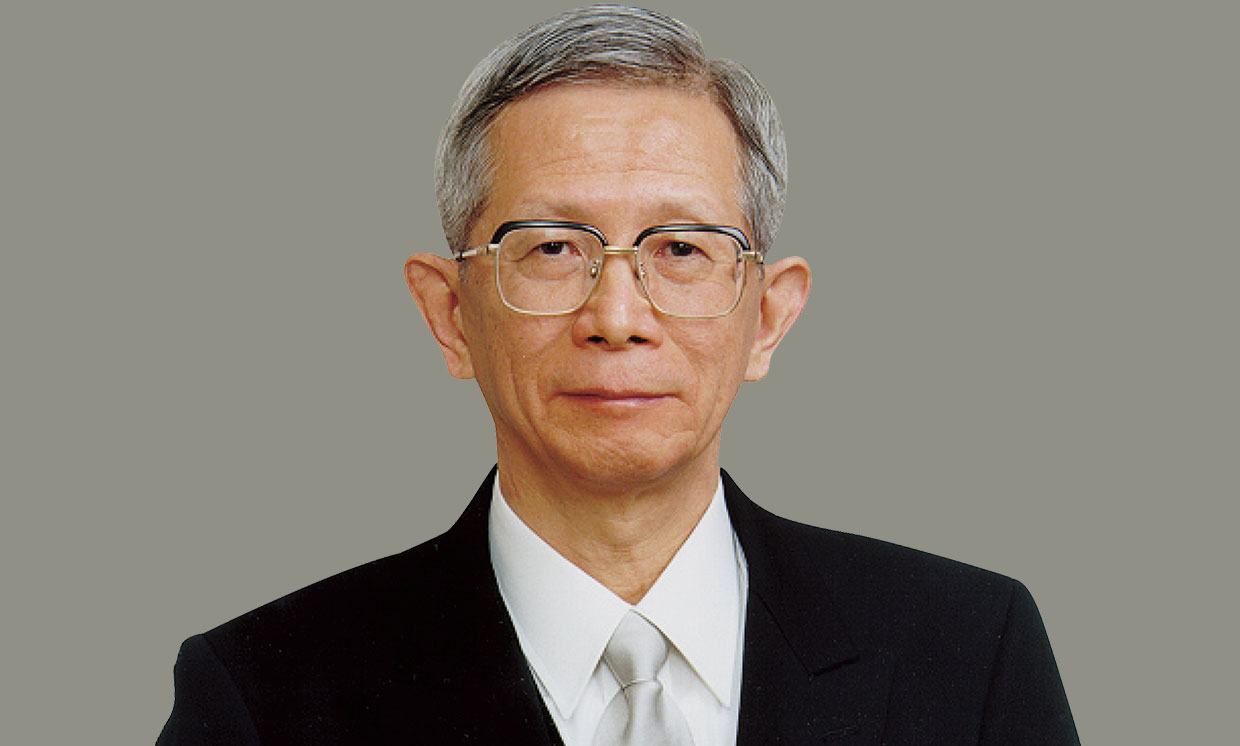
\includegraphics[width=120mm , angle = 0  ]{Aoyagi.jpg}}
	\caption{Sideways figure.}
	\label{f5}
\end{sidewaysfigure}



